% Options for packages loaded elsewhere
\PassOptionsToPackage{unicode}{hyperref}
\PassOptionsToPackage{hyphens}{url}
\PassOptionsToPackage{dvipsnames,svgnames,x11names}{xcolor}
\PassOptionsToPackage{space}{xeCJK}
\documentclass[
  10pt,
  a4paper,
]{article}
\usepackage{xcolor}
\usepackage[top=18mm,bottom=18mm,left=20mm,right=20mm]{geometry}
\usepackage{amsmath,amssymb}
\setcounter{secnumdepth}{-\maxdimen} % remove section numbering
\usepackage{iftex}
\ifPDFTeX
  \usepackage[T1]{fontenc}
  \usepackage[utf8]{inputenc}
  \usepackage{textcomp} % provide euro and other symbols
\else % if luatex or xetex
  \usepackage{unicode-math} % this also loads fontspec
  \defaultfontfeatures{Scale=MatchLowercase}
  \defaultfontfeatures[\rmfamily]{Ligatures=TeX,Scale=1}
\fi
\usepackage{lmodern}
\ifPDFTeX\else
  % xetex/luatex font selection
  \setmainfont[]{Times New Roman}
  \setsansfont[]{Arial}
  \setmonofont[]{Menlo}
  \ifXeTeX
    \usepackage{xeCJK}
    \setCJKmainfont[]{Songti SC}
  \fi
  \ifLuaTeX
    \usepackage[]{luatexja-fontspec}
    \setmainjfont[]{Songti SC}
  \fi
\fi
% Use upquote if available, for straight quotes in verbatim environments
\IfFileExists{upquote.sty}{\usepackage{upquote}}{}
\IfFileExists{microtype.sty}{% use microtype if available
  \usepackage[]{microtype}
  \UseMicrotypeSet[protrusion]{basicmath} % disable protrusion for tt fonts
}{}
\makeatletter
\@ifundefined{KOMAClassName}{% if non-KOMA class
  \IfFileExists{parskip.sty}{%
    \usepackage{parskip}
  }{% else
    \setlength{\parindent}{0pt}
    \setlength{\parskip}{6pt plus 2pt minus 1pt}}
}{% if KOMA class
  \KOMAoptions{parskip=half}}
\makeatother
\usepackage{color}
\usepackage{fancyvrb}
\newcommand{\VerbBar}{|}
\newcommand{\VERB}{\Verb[commandchars=\\\{\}]}
\DefineVerbatimEnvironment{Highlighting}{Verbatim}{commandchars=\\\{\}}
% Add ',fontsize=\small' for more characters per line
\newenvironment{Shaded}{}{}
\newcommand{\AlertTok}[1]{\textcolor[rgb]{1.00,0.00,0.00}{\textbf{#1}}}
\newcommand{\AnnotationTok}[1]{\textcolor[rgb]{0.38,0.63,0.69}{\textbf{\textit{#1}}}}
\newcommand{\AttributeTok}[1]{\textcolor[rgb]{0.49,0.56,0.16}{#1}}
\newcommand{\BaseNTok}[1]{\textcolor[rgb]{0.25,0.63,0.44}{#1}}
\newcommand{\BuiltInTok}[1]{\textcolor[rgb]{0.00,0.50,0.00}{#1}}
\newcommand{\CharTok}[1]{\textcolor[rgb]{0.25,0.44,0.63}{#1}}
\newcommand{\CommentTok}[1]{\textcolor[rgb]{0.38,0.63,0.69}{\textit{#1}}}
\newcommand{\CommentVarTok}[1]{\textcolor[rgb]{0.38,0.63,0.69}{\textbf{\textit{#1}}}}
\newcommand{\ConstantTok}[1]{\textcolor[rgb]{0.53,0.00,0.00}{#1}}
\newcommand{\ControlFlowTok}[1]{\textcolor[rgb]{0.00,0.44,0.13}{\textbf{#1}}}
\newcommand{\DataTypeTok}[1]{\textcolor[rgb]{0.56,0.13,0.00}{#1}}
\newcommand{\DecValTok}[1]{\textcolor[rgb]{0.25,0.63,0.44}{#1}}
\newcommand{\DocumentationTok}[1]{\textcolor[rgb]{0.73,0.13,0.13}{\textit{#1}}}
\newcommand{\ErrorTok}[1]{\textcolor[rgb]{1.00,0.00,0.00}{\textbf{#1}}}
\newcommand{\ExtensionTok}[1]{#1}
\newcommand{\FloatTok}[1]{\textcolor[rgb]{0.25,0.63,0.44}{#1}}
\newcommand{\FunctionTok}[1]{\textcolor[rgb]{0.02,0.16,0.49}{#1}}
\newcommand{\ImportTok}[1]{\textcolor[rgb]{0.00,0.50,0.00}{\textbf{#1}}}
\newcommand{\InformationTok}[1]{\textcolor[rgb]{0.38,0.63,0.69}{\textbf{\textit{#1}}}}
\newcommand{\KeywordTok}[1]{\textcolor[rgb]{0.00,0.44,0.13}{\textbf{#1}}}
\newcommand{\NormalTok}[1]{#1}
\newcommand{\OperatorTok}[1]{\textcolor[rgb]{0.40,0.40,0.40}{#1}}
\newcommand{\OtherTok}[1]{\textcolor[rgb]{0.00,0.44,0.13}{#1}}
\newcommand{\PreprocessorTok}[1]{\textcolor[rgb]{0.74,0.48,0.00}{#1}}
\newcommand{\RegionMarkerTok}[1]{#1}
\newcommand{\SpecialCharTok}[1]{\textcolor[rgb]{0.25,0.44,0.63}{#1}}
\newcommand{\SpecialStringTok}[1]{\textcolor[rgb]{0.73,0.40,0.53}{#1}}
\newcommand{\StringTok}[1]{\textcolor[rgb]{0.25,0.44,0.63}{#1}}
\newcommand{\VariableTok}[1]{\textcolor[rgb]{0.10,0.09,0.49}{#1}}
\newcommand{\VerbatimStringTok}[1]{\textcolor[rgb]{0.25,0.44,0.63}{#1}}
\newcommand{\WarningTok}[1]{\textcolor[rgb]{0.38,0.63,0.69}{\textbf{\textit{#1}}}}
\usepackage{longtable,booktabs,array}
\usepackage{calc} % for calculating minipage widths
% Correct order of tables after \paragraph or \subparagraph
\usepackage{etoolbox}
\makeatletter
\patchcmd\longtable{\par}{\if@noskipsec\mbox{}\fi\par}{}{}
\makeatother
% Allow footnotes in longtable head/foot
\IfFileExists{footnotehyper.sty}{\usepackage{footnotehyper}}{\usepackage{footnote}}
\makesavenoteenv{longtable}
\usepackage{graphicx}
\makeatletter
\newsavebox\pandoc@box
\newcommand*\pandocbounded[1]{% scales image to fit in text height/width
  \sbox\pandoc@box{#1}%
  \Gscale@div\@tempa{\textheight}{\dimexpr\ht\pandoc@box+\dp\pandoc@box\relax}%
  \Gscale@div\@tempb{\linewidth}{\wd\pandoc@box}%
  \ifdim\@tempb\p@<\@tempa\p@\let\@tempa\@tempb\fi% select the smaller of both
  \ifdim\@tempa\p@<\p@\scalebox{\@tempa}{\usebox\pandoc@box}%
  \else\usebox{\pandoc@box}%
  \fi%
}
% Set default figure placement to htbp
\def\fps@figure{htbp}
\makeatother
\setlength{\emergencystretch}{3em} % prevent overfull lines
\providecommand{\tightlist}{%
  \setlength{\itemsep}{0pt}\setlength{\parskip}{0pt}}
\usepackage{float}
\usepackage{caption}
\floatplacement{figure}{H}
\captionsetup{font=small,skip=4pt}
\renewcommand{\figurename}{图}
\renewcommand{\tablename}{表}
\setlength{\parskip}{4pt}
\setlength{\parindent}{0pt}
\setlength{\textfloatsep}{8pt}
\setlength{\intextsep}{8pt}
\setlength{\tabcolsep}{5pt}
\renewcommand{\arraystretch}{1.12}
\setcounter{secnumdepth}{0}
\AtBeginDocument{\fontsize{10.5}{14}\selectfont}
\usepackage{bookmark}
\IfFileExists{xurl.sty}{\usepackage{xurl}}{} % add URL line breaks if available
\urlstyle{same}
\hypersetup{
  colorlinks=true,
  linkcolor={Maroon},
  filecolor={Maroon},
  citecolor={Blue},
  urlcolor={blue},
  pdfcreator={LaTeX via pandoc}}

\author{}
\date{}

\begin{document}

\section{OpenMP CSR SpMV
并行策略实验报告}\label{openmp-csr-spmv-ux5e76ux884cux7b56ux7565ux5b9eux9a8cux62a5ux544a}

\subsection{1.
实验目标与策略设计}\label{ux5b9eux9a8cux76eeux6807ux4e0eux7b56ux7565ux8bbeux8ba1}

CSR 稀疏矩阵向量乘按行计算
\(y_i=\sum_{p=row\_ptr[i]}^{row\_ptr[i+1]-1}values[p]\,x[col\_idx[p]]\)。不同行的输出独立，但行长偏斜会使等量行数对应不同工作量。本实验研究：按行动态调度能否改善偏斜负载，按
NNZ 划分能否拆开长行，以及更细的动态 NNZ 块是否值得额外调度开销。

\begin{longtable}[]{@{}llcc@{}}
\toprule\noalign{}
实现 & 工作划分与调度 & 长行可拆分 & 段内 SIMD \\
\midrule\noalign{}
\endhead
\bottomrule\noalign{}
\endlastfoot
student1 & 按行 \texttt{schedule(static)} & 否 & 否 \\
student2 & 按行 \texttt{schedule(dynamic,128)} & 否 & 否 \\
student3 & 每个实际线程固定一个连续 NNZ 块 & 是 & 是 \\
student4 & 约每个请求线程 4 个 NNZ 块，\texttt{dynamic,1} & 是 & 是 \\
\end{longtable}

\texttt{student1} 开销小，但长行可能集中在某个线程；\texttt{student2}
动态领取 128
行一组的任务，兼顾均衡与领取开销，但仍无法拆开单条长行。\texttt{student3}
将非零数组均分为 \(P\) 个区间，每线程自行通过 \texttt{upper\_bound}
找到对应行；完整行直接写输出，边界行先保存部分和，退出并行区后按块编号合并。每块至多记录两个边界行，因此无需对每个乘加使用原子操作。

\texttt{student4} 延用相同计算与合并代码，将块数增至约
\(4P\)，使先完成的线程可以继续领块。这里 \texttt{dynamic,1} 的一个任务是
NNZ 块，而不是一行；请求 8 线程时，默认矩阵约分成 32 块，每块约 3 万
NNZ。NNZ 很少时限制块数，全空矩阵保留一个块。

\subsection{2.
环境、参数与测量方法}\label{ux73afux5883ux53c2ux6570ux4e0eux6d4bux91cfux65b9ux6cd5}

硬件为 MacBook Air、Apple M5、24 GB 内存，10 个 CPU 核心（4 个性能核、6
个能效核）；系统 macOS 26.5.2，编译器 Apple Clang 21.0.0，OpenMP 运行库
Homebrew libomp 23.1.2。所有策略统一使用
\texttt{-O2\ -std=c++17\ -pthread}，通过
\texttt{-Xpreprocessor\ -fopenmp} 和 \texttt{-lomp} 启用 OpenMP；未使用
\texttt{-O3}、\texttt{-march=native} 或
\texttt{-ffast-math}，未设置线程绑定。

默认矩阵为 10000 行、100000 列，普通行 32 NNZ，32 条长行各 20000 NNZ，总
NNZ 为 958976，随机种子为 20260926。研究线程数
1、2、4、8、10，另外改变规模、偏斜程度、调度及随机种子。每个配置进行 10
轮实验，每轮各策略预热一次、验证结果后计时 100 次，使用
\texttt{steady\_clock}；轮内策略顺序随机打乱。报告采用每轮平均耗时的中位数，原始数据同时保存最小值和最大值。

矩阵生成、随机数、正确性检查和打印不计入计时；线程创建回收、NNZ
临时数组分配、边界搜索、同步与合并均计入。所有输入、编译选项及计时范围对各策略一致。

加速比定义为 \(S_P=T_s/T_P\)，并行效率为 \(E_P=S_P/P\)，其中 \(T_s\)
始终指纯串行基线。默认矩阵线程扩展分析固定采用 \texttt{default\_t1}
中的串行中位数 \textbf{0.668883 ms}，避免随线程档位更换分母。

正确性保留原串行参考与 \(10^{-10}\)
绝对、相对误差判定。所有正式策略通过报告测量中的检查；NNZ 两策略另通过
7524 次边界与随机矩阵检查，包括空行、全空、线程数多于
NNZ、单行跨多个块及更换向量后重复调用。优化构建、地址/未定义行为检查、实际线程数受限及关闭
OpenMP 的回退运行均通过。拆行与 SIMD
会改变浮点累加顺序，未放宽误差标准。

\newpage

\subsection{3.
默认矩阵性能与线程扩展}\label{ux9ed8ux8ba4ux77e9ux9635ux6027ux80fdux4e0eux7ebfux7a0bux6269ux5c55}

下表为默认矩阵 8 线程结果，时间单位 ms；串行基线取上一节固定值。

\begin{longtable}[]{@{}lrrr@{}}
\toprule\noalign{}
实现 & 中位耗时 & 加速比 \(S_8\) & 效率 \(E_8\) \\
\midrule\noalign{}
\endhead
\bottomrule\noalign{}
\endlastfoot
serial & 0.6689 & 1.00 & 不适用 \\
std::thread & 0.2400 & 2.79 & 34.8\% \\
student1 & 0.1805 & 3.71 & 46.3\% \\
student2 & 0.1761 & 3.80 & 47.5\% \\
student3 & 0.1629 & 4.11 & 51.3\% \\
student4 & 0.1407 & 4.75 & 59.4\% \\
\end{longtable}

\texttt{student2} 相对 \texttt{student1} 改善约
2.4\%，本次配置中收益有限；NNZ 固定块加入拆行及 SIMD
后进一步改善。\texttt{student4} 比 \texttt{student3} 耗时降低
\textbf{13.6\%}，比 \texttt{student2} 降低
\textbf{20.1\%}。这些是同一次统一测量的结果，不与早期优化数据混算。

\begin{longtable}[]{@{}
  >{\raggedleft\arraybackslash}p{(\linewidth - 8\tabcolsep) * \real{0.2000}}
  >{\raggedleft\arraybackslash}p{(\linewidth - 8\tabcolsep) * \real{0.2000}}
  >{\raggedleft\arraybackslash}p{(\linewidth - 8\tabcolsep) * \real{0.2000}}
  >{\raggedleft\arraybackslash}p{(\linewidth - 8\tabcolsep) * \real{0.2000}}
  >{\raggedleft\arraybackslash}p{(\linewidth - 8\tabcolsep) * \real{0.2000}}@{}}
\toprule\noalign{}
\begin{minipage}[b]{\linewidth}\raggedleft
线程数 \(P\)
\end{minipage} & \begin{minipage}[b]{\linewidth}\raggedleft
student3 时间
\end{minipage} & \begin{minipage}[b]{\linewidth}\raggedleft
student4 时间
\end{minipage} & \begin{minipage}[b]{\linewidth}\raggedleft
student4 加速比
\end{minipage} & \begin{minipage}[b]{\linewidth}\raggedleft
student4 效率
\end{minipage} \\
\midrule\noalign{}
\endhead
\bottomrule\noalign{}
\endlastfoot
1 & 0.5061 & 0.5089 & 1.31 & 131.4\% \\
2 & 0.2610 & 0.2636 & 2.54 & 126.9\% \\
4 & 0.1544 & 0.1606 & 4.16 & 104.1\% \\
8 & 0.1629 & 0.1407 & 4.75 & 59.4\% \\
10 & 0.1680 & 0.1392 & 4.81 & 48.1\% \\
\end{longtable}

\begin{figure}
\centering
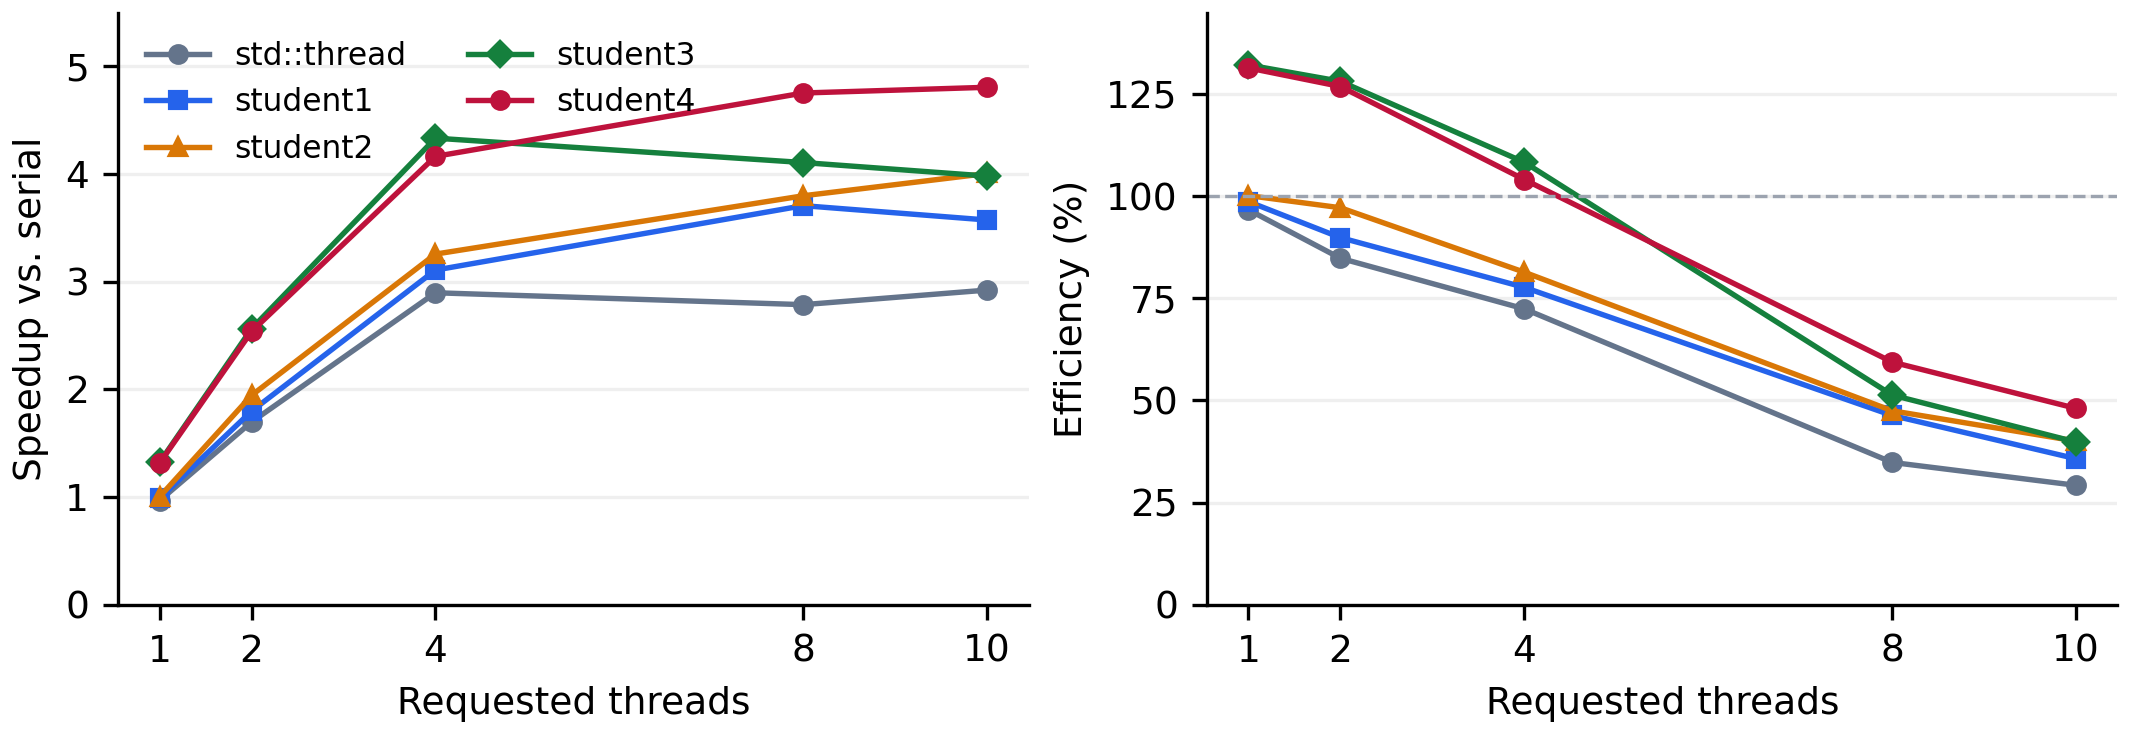
\includegraphics[width=16.8cm,height=\textheight,keepaspectratio,alt={默认矩阵的加速比与并行效率。分母固定为纯串行基线；NNZ 策略包含 SIMD，低线程数效率超过 100\% 不等于线程调度实现了超线性扩展。}]{assets/scaling.png}
\caption{默认矩阵的加速比与并行效率。分母固定为纯串行基线；NNZ 策略包含
SIMD，低线程数效率超过 100\% 不等于线程调度实现了超线性扩展。}
\end{figure}

\texttt{student3} 从 4 扩至 8、10 线程反而变慢；\texttt{student4}
能继续小幅改善，但 8 到 10 线程的收益仅约 1.1\%，效率明显下降。SIMD
策略在单线程下也快于原串行，故上述效率不能仅用于评价线程扩展能力。若以
\texttt{student4} 自身单线程时间为参照，其 10 线程扩展比为
\textbf{3.66}，相应效率约 \textbf{36.6\%}。

两种线程 API 都适合按行独立计算。当前 \texttt{std::thread}
基线每次调用都创建并回收线程，OpenMP
运行时通常可复用工作线程，因而短任务开销不同；\texttt{student4}
比该基线快约 \textbf{41.4\%}，但这同时包含工作划分与 SIMD
的影响，不能全部归因于线程复用。OpenMP
简化循环调度；自定义线程池、任务队列、线程间通信及线程生命周期控制则更适合采用
\texttt{std::thread}。本实验未改造线程池基线。

\newpage

\subsection{4.
规模、偏斜与随机性}\label{ux89c4ux6a21ux504fux659cux4e0eux968fux673aux6027}

以下配置均为 8 线程，时间单位 ms。A：普通行 1 NNZ、仅 1 条长行 100000
NNZ；B：无长行，其余默认；C：20000 行、200000 列、普通行 16 NNZ、16
条长行各 80000 NNZ；D/E：默认矩阵，种子改为 7/42。

\begin{longtable}[]{@{}lrrrr@{}}
\toprule\noalign{}
配置 & student1 & student2 & student3 & student4 \\
\midrule\noalign{}
\endhead
\bottomrule\noalign{}
\endlastfoot
A：单条长行占主导 & 0.1049 & 0.0946 & 0.0359 & 0.0376 \\
B：均匀短行 & 0.0674 & 0.0667 & 0.0656 & 0.0646 \\
C：较大偏斜矩阵 & 0.4652 & 0.2744 & 0.2583 & 0.2262 \\
D：seed=7 & 0.2034 & 0.1917 & 0.1772 & 0.1424 \\
E：seed=42 & 0.2081 & 0.1738 & 0.1698 & 0.1437 \\
\end{longtable}

A 中按行策略无法协同处理唯一长行，NNZ
拆分优势突出；但细分动态块的收益不足以抵消开销，\texttt{student4} 比
\texttt{student3} 慢约 \textbf{4.8\%}，是负优化案例。默认 4
线程下也存在类似现象。B
中策略差距很小，均匀短行没有明显的负载均衡需求。C 中 \texttt{student4}
比 \texttt{student3} 快 \textbf{12.4\%}；C
同时改变规模和偏斜，只作为组合压力测试，不用于隔离某一变量的贡献。D/E
中该收益约为
\textbf{19.6\%/15.4\%}，说明改善不只出现在默认种子，但不能据此推广到任意稀疏矩阵。

\subsection{5.
消融：小块数量与动态调度}\label{ux6d88ux878dux5c0fux5757ux6570ux91cfux4e0eux52a8ux6001ux8c03ux5ea6}

采用独立的 NNZ 调度驱动，保持相同乘加、SIMD
及部分和合并，只改变块数和调度；默认矩阵、8 线程、10 轮，每轮 100
次。该实验与正文统一测量属于不同运行批次，以下数值只在本组内部比较。

\begin{figure}
\centering
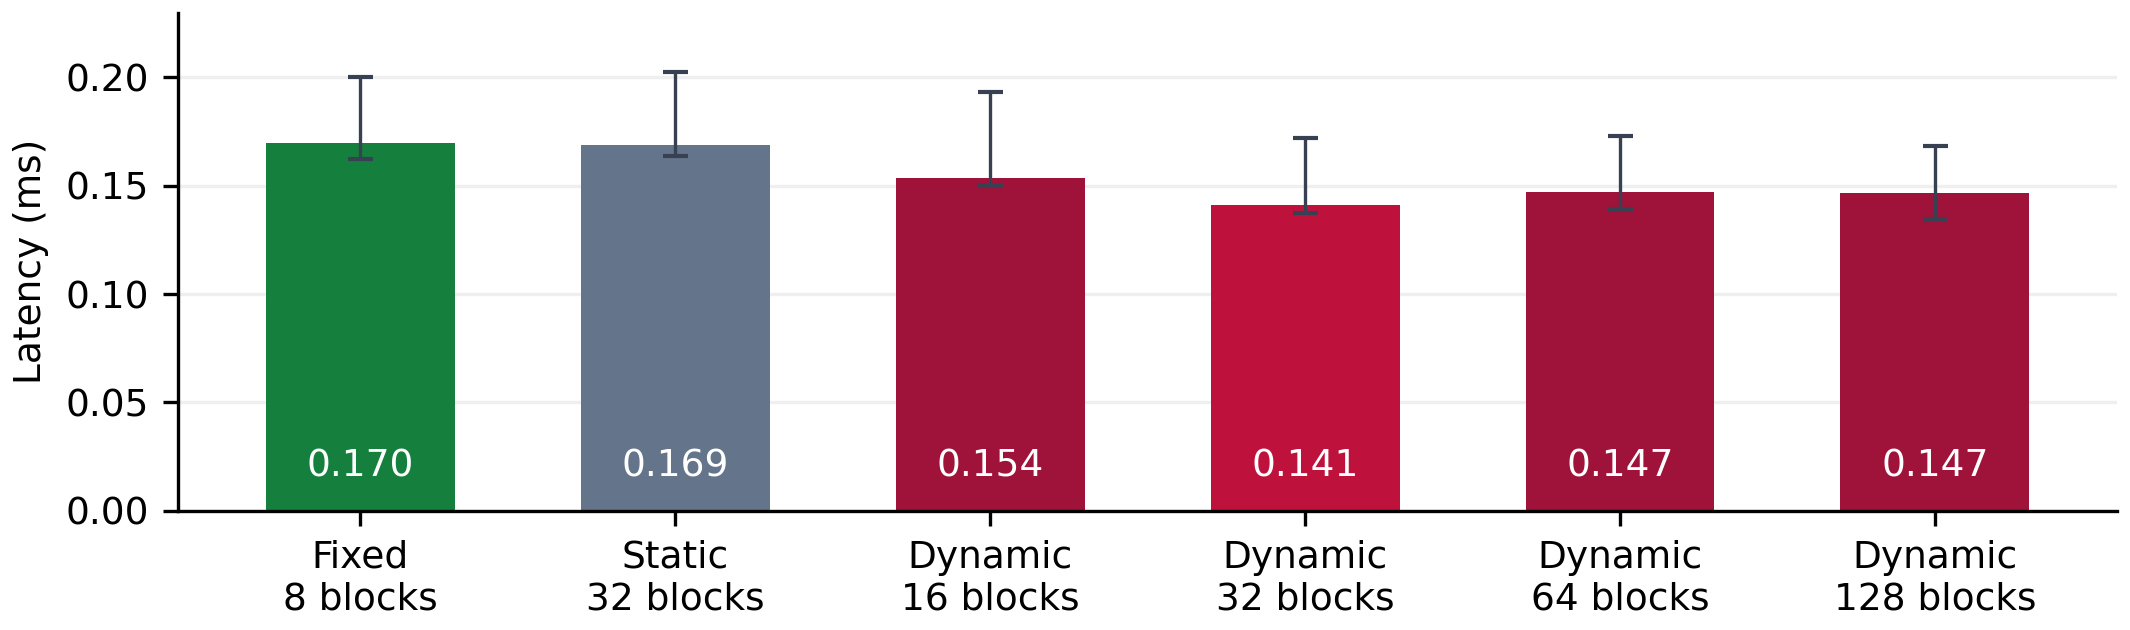
\includegraphics[width=16.8cm,height=\textheight,keepaspectratio,alt={NNZ 调度消融。柱高为中位数，误差线为 10 轮中的最小值至最大值；它不是置信区间。}]{assets/ablation.png}
\caption{NNZ 调度消融。柱高为中位数，误差线为 10
轮中的最小值至最大值；它不是置信区间。}
\end{figure}

固定 8 块为 0.169632 ms；划成 32 个 static 块为 0.168885
ms，单纯细分收益很小。相同的 32 块采用 dynamic 后降至 0.141329
ms，支持动态领取任务能减少本例等待时间的解释。16、64、128 个 dynamic
块分别为 0.153695、0.147112、0.146650
ms；块越多并未持续改善，领取任务、边界查找、部分和写入及合并开销需要权衡，因此选择每线程约
4 块。

此外，早期 NNZ 策略消融中，默认 8 线程的无 SIMD 精确切块为 0.196690
ms，加入 SIMD 后为 0.163355
ms。该独立实验以及正文单线程结果表明，段内累加优化确实贡献了收益，不能将
NNZ 策略的全部加速解释为负载均衡。

\newpage

\subsection{6. Linux
perf：未完成的测量}\label{linux-perfux672aux5b8cux6210ux7684ux6d4bux91cf}

\textbf{本报告尚未包含作业要求的 Linux \texttt{perf\ stat} 数据。}
当前测量环境为 macOS，暂无法使用可用的 Linux 测量环境，因此
\texttt{cycles}、\texttt{instructions}、\texttt{cache-misses}、上下文切换和
CPU 迁移等事件均未采集。本节明确记录缺项，不用运行时间推算硬件计数器。

已有实验支持``动态 NNZ
小块在部分配置上更快''，但不能确定线程扩展下降主要来自内存带宽、缓存失效、异构核心调度还是运行时开销。后续在
Linux 上应对纯串行、原始 \texttt{std::thread} 和一个 OpenMP
策略分别测量；需要单策略入口，避免把同时执行多个策略的计数器归因给某个内核。Linux
环境数据也应单独标注，不能与本机 M5 时间直接混算。

\subsection{7. 结论与局限}\label{ux7ed3ux8bbaux4e0eux5c40ux9650}

按行 static 的优势是简单和调度开销小；按行 dynamic
可缓解行间不均衡，但不能拆开单条长行。NNZ 拆分加 SIMD
对强偏斜输入更有效；动态小块进一步改善了默认 8
线程及组合压力配置，但在低线程数、任务较小或已有负载均衡时可能负优化。最终保留四种策略以展示这些权衡。

默认矩阵中 \texttt{student4} 达到 0.1407 ms（8
线程），相对固定纯串行基线为 4.75 倍加速；增加至 10 线程达到 0.1392
ms，加速 4.81 倍，但边际收益很小。当前均分模型只考虑
NNZ，没有包含每行固定开销；随机读取
\texttt{x}、缓存行为、内存带宽及线程运行速度仍可能影响性能。每线程 4
块是本机经验参数，不能保证跨机器最优。

实验局限还包括：只有合成 CSR 输入，未测试真实矩阵数据集；未固定 CPU
频率或绑定线程；10 轮存在离散波动，未进行显著性检验；尚缺 Linux
\texttt{perf} 数据。报告中的解释以测量支持的范围为限。

\subsection{8. 可复现性、AI
使用与参考资料}\label{ux53efux590dux73b0ux6027ai-ux4f7fux7528ux4e0eux53c2ux8003ux8d44ux6599}

当前最终代码的统一实验驱动为
\texttt{report/benchmark\_report.cpp}，配置脚本为
\texttt{report/measure\_report.py}，原始与汇总数据为
\texttt{report/measurements\_raw.csv}、\texttt{report/measurements\_summary.csv}。NNZ
调度消融数据位于 \texttt{experiments/nnz\_schedules\_*.csv}，早期 SIMD
消融见 \texttt{student3\_optimization.md}，数据备份在
\texttt{report/supplement/}。最小值与最大值保留在
CSV，核心结论已在正文给出。

学生完成 \texttt{student1}、\texttt{student2} 及初版
\texttt{student3}；OpenAI Codex 协助后续 NNZ
优化设计、实现、验证、实验脚本、图表及本报告初稿。正式提交前由学生核实数据、代码和结论，并按要求附相关对话截图。心路历程报告另由学生本人撰写，本文不代写该部分。

参考资料：

\begin{enumerate}
\def\labelenumi{\arabic{enumi}.}
\tightlist
\item
  课程作业文档《实验一：OpenMP CSR SpMV 并行编程》及项目
  \texttt{README.md}。
\item
  OpenMP ARB.
  \href{https://www.openmp.org/wp-content/uploads/OpenMP-API-Specification-5-2.pdf}{OpenMP
  API Specification 5.2}，parallel、worksharing-loop、schedule 与 simd
  reduction。
\item
  cppreference.
  \href{https://en.cppreference.com/w/cpp/thread/thread.html}{std::thread}。
\item
  Linux manual pages.
  \href{https://man7.org/linux/man-pages/man1/perf-stat.1.html}{perf-stat(1)}。
\end{enumerate}

\newpage

\section{附录
A：正确性证据与复现}\label{ux9644ux5f55-aux6b63ux786eux6027ux8bc1ux636eux4e0eux590dux73b0}

下面为学生已有的早期 \texttt{student1}/\texttt{student2}
运行截图。截图时间属于早期探索，不参与正文最终版本的定量比较，也不作为
\texttt{student3}/\texttt{student4} 的验证证据。

\begin{figure}
\centering
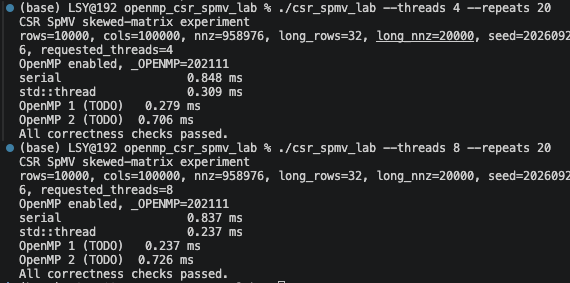
\includegraphics[width=14.5cm,height=\textheight,keepaspectratio,alt={早期两种按行策略在 4、8 线程下通过正确性检查。}]{assets/early_correctness.png}
\caption{早期两种按行策略在 4、8 线程下通过正确性检查。}
\end{figure}

最终 NNZ 策略的 \texttt{experiments/check\_nnz\_strategies.cpp}
每次先把输出填为 NaN，再检查所有行有限且满足原误差判定。两个策略各 3762
次、共 7524
次检查，正式优化构建、地址/未定义行为检查构建、\texttt{OMP\_DYNAMIC=true\ OMP\_THREAD\_LIMIT=2}
运行和关闭 OpenMP 的回退分别通过。地址检查构建未成功向量化，故另用正式
\texttt{-O2} 构建验证 SIMD 数值结果。

在项目根目录复现正文数据：

\begin{Shaded}
\begin{Highlighting}[]
\FunctionTok{clang}\NormalTok{++ }\AttributeTok{{-}O2} \AttributeTok{{-}std}\OperatorTok{=}\NormalTok{c++17 }\AttributeTok{{-}Xpreprocessor} \AttributeTok{{-}fopenmp} \DataTypeTok{\textbackslash{}}
  \AttributeTok{{-}I}\NormalTok{/opt/homebrew/opt/libomp/include }\DataTypeTok{\textbackslash{}}
  \AttributeTok{{-}L}\NormalTok{/opt/homebrew/opt/libomp/lib }\DataTypeTok{\textbackslash{}}
  \AttributeTok{{-}Wl,{-}rpath,}\NormalTok{/opt/homebrew/opt/libomp/lib }\DataTypeTok{\textbackslash{}}
  \AttributeTok{{-}lomp} \AttributeTok{{-}pthread}\NormalTok{ report/benchmark\_report.cpp }\DataTypeTok{\textbackslash{}}
  \AttributeTok{{-}o}\NormalTok{ /private/tmp/spmv\_report\_bench}
\ExtensionTok{python3}\NormalTok{ report/measure\_report.py /private/tmp/spmv\_report\_bench}
\end{Highlighting}
\end{Shaded}

正文图表由 \texttt{report/make\_figures.py} 读取 CSV
生成。调度消融的复现命令见
\texttt{experiments/README.md}。最终源码中共注册四个 OpenMP
策略，均经过原 \texttt{benchmark\_ms} 的预热及正确性检查。

\end{document}
